\chapter{Hadoop Internals}
	\subsubsection{Terminology}
	\par
		A \textbf{Job} is an execution of a mapper and reducer across a data set.
		\newline
		A \textbf{Task} is an execution of a mapper or a reducer on a slice of data.
		\newline
		A \textbf{Task Attempt} is an instance of an attempt to execute a task\footnote{Tasks attempt at least once, possibly more. Multiple crashes on input imply discarding it. Multiple attempts may occur in parallel (speculative execution), the TaskID is not a unique identifier.}.
\section{Hadoop Distributed File System}
	\subsection{Motivations}
	\par
		As dataset size increase, more computing capacity is required for processing and, as computing capacity grows, the link between the computing nodes and the storage nodes becomes a bottleneck.
		\newline
		Special-purpose interconnections for high performance computing are a costly solution, a distributed file system is not mandatory but highly desirable.
		\newline
	\par
		The key idea is to abandon the separation between compute and storage nodes: \textbf{large datasets are partitioned across a number of separate (commodity) machines} in a network-based system with all its complications (failure tolerance).
		\newline
		Distributes file systems for MapReduce are built upon previous results with different requirements: \textbf{write once, read many workloads} (do not handle concurrency but allow replication). They are optimized for throughput, not for latency.
	\subsection{Blocks}
	\par
		Files are broken into big [64, 128] MB block-sized chunks\footnote{Files smaller than a single block do not occupy a full block's worth of underlying storage.} to \textbf{make transfer times larger than seek latency}, this also avoids problems related to metadata management.
	\par
		Blocks are stored on independent machines and replicated across the local disks of nodes in the cluster (reliability and parallel access), replication is handled by storage nodes themselves.
	\subsection{Architecture}
		\par\indent
		\par\indent\textbf{Namenode}: Keeps metadata in RAM (150 bytes for each block). Persistence of metadata depends on synchronous and atomic writes to NFS. Maintains overall \textbf{health} of the file system.
		\par
		\textbf{Secondary NodeName}: It merges the namespace with the edit log. To recover from a failure of a NameNode, use the NFS copy of metadata and switch the secondary to primary.
		\par
		\textbf{DataNode}: They store data and talk to clients. They report periodically to the NameNode the list of blocks the hold.
		\begin{figure}[h!]
			\centering
			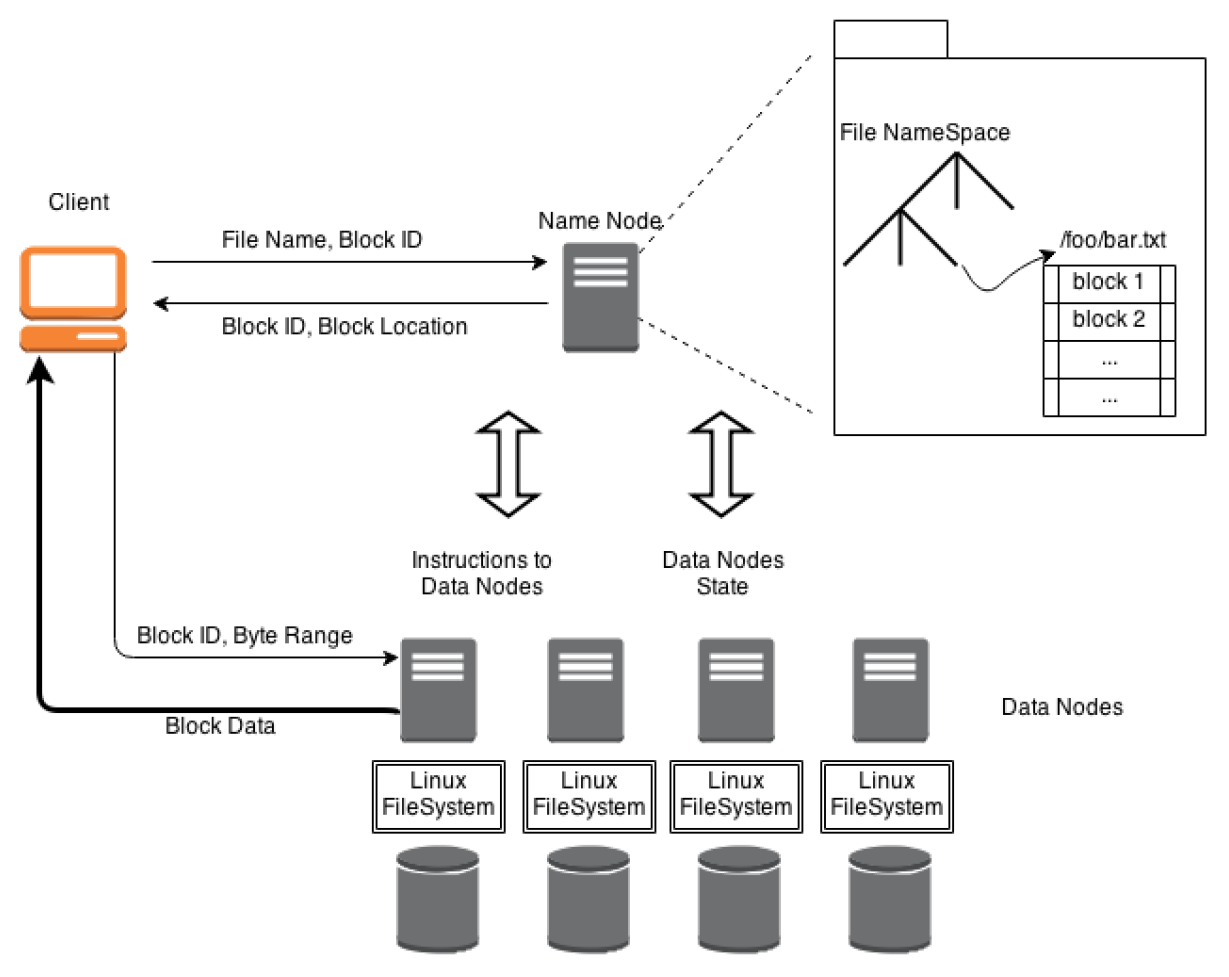
\includegraphics[width=0.8\linewidth]{images/arch_sketch.png}
			\caption{\textit{Architecture sketch of HDFS operations.}}
		\end{figure}
	\subsubsection{File read}
		\par
		The NameNode is only used to get the block location. Unresponsive DataNodes are discarded by clients.
		\newline
		To external clients, for each block, the namenode returne a set of datanodes sorted according to their proximity to the client.
		\newline
		To MapReduce clients, TaskTracker and DataNodes are collocated and, for each block, the namenode usually returns the local DataNode.
	\subsubsection{File write}
		\par
		The client asks the NameNode for a list of suitable DataNodes, the list forms a pipeline: the first DataNode stores a copy of a block, then forwards it to the second, and so on (\textbf{replication}).
		\newline
		The \textbf{replica placement is a trade-off between reliability and bandwidth}, the default placement requires a copy on the same node of the client, a replica \textbf{off-rack} and another on the same rack as the second but on a different node.
	\subsubsection{HDFS coherency model}
		\par
		The namespace is updates but the block contents may not be visible after a write is finished. To force synchronization it is necessary to use \textit{sync()}, but it involves some overhead (trade-off between robustness/consistency and throughput).
		\newline
		Multiple writers for the same block are not supported but different block can be written in parallel by using MapReduce.

\section[Hadhoop MapReduce]{Hadhoop MapReduce\protect\footnotemark}
\footnotetext{MapReduce APIs are evolving fast, therefore it is advised to use the appropriate API documentation and Eclipse instead of the prof notes.}
	\subsection{Anatomy of a job run}
		\begin{figure}[h!]
			\centering
			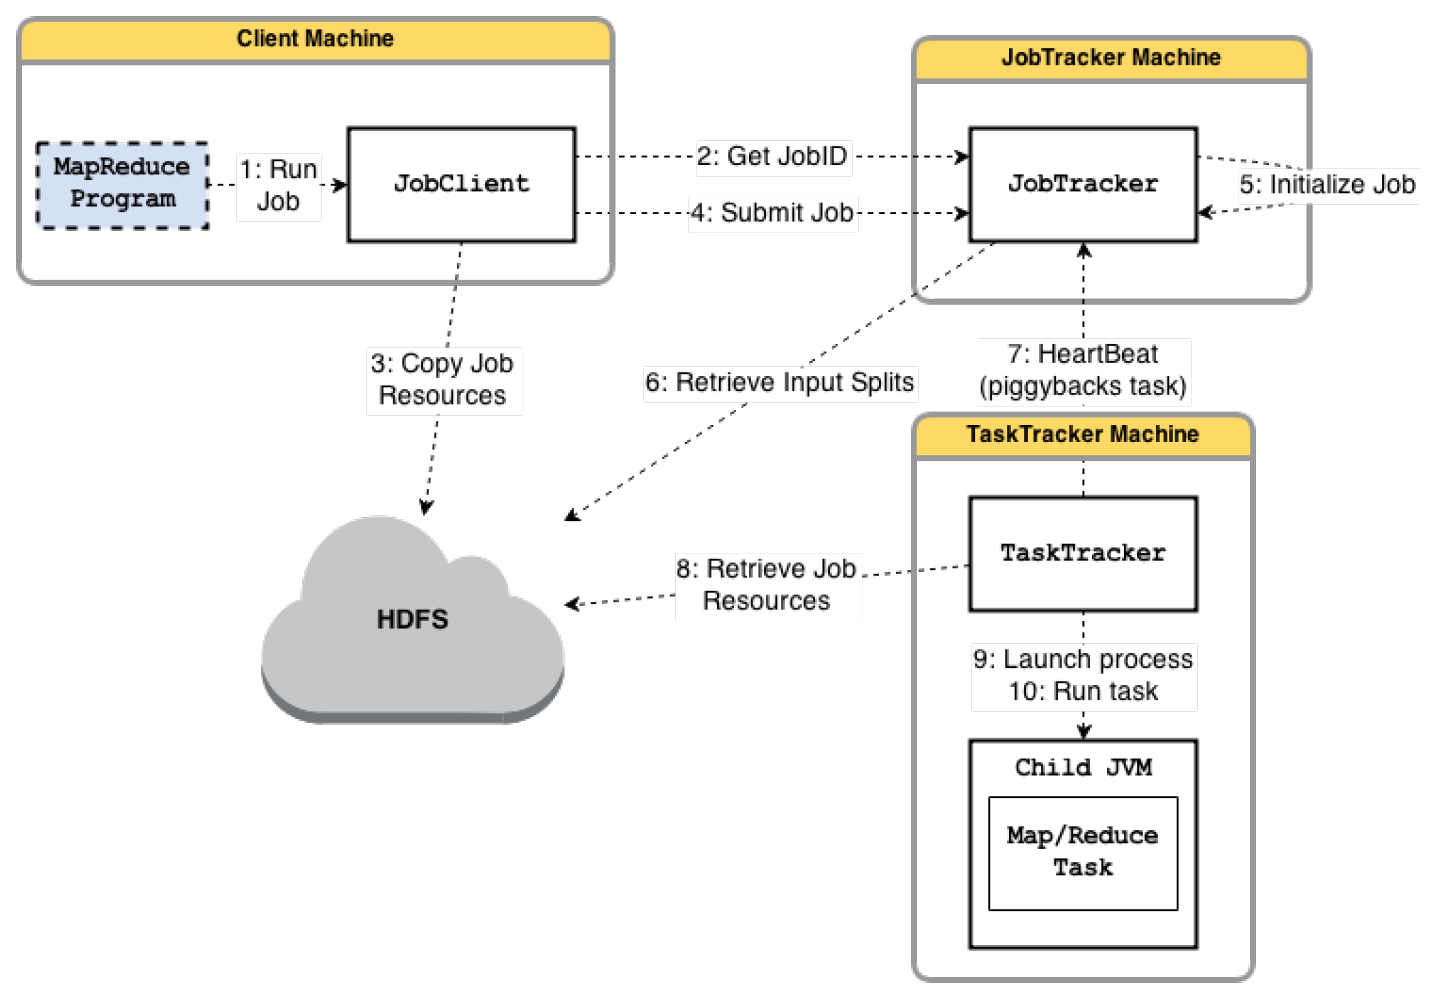
\includegraphics[width=\linewidth]{images/jobrun.png}
			\caption{\textit{Anatomy of a MapReduce job run.}}
		\end{figure}
	\subsubsection{Job submission}
		\par
		The \textit{runJob()} method creates a new instance of a \textbf{JobClient}, then it calls \textit{submitJob()} on this class.
		\newline
		Some simple verifications are done on the job to check if there is an output directory, input splits, and if the JAR of the job can be copied to the HDFS\footnote{The JAR of the job is replicated 10 times}.
	\subsubsection{Job initialization}
		\par
		The \textbf{JobTracker} is responsible for the creation of an object for the job. It encapsulates its tasks and does the \textbf{bookkeeping} with the tasks' status and progress.
		\newline
		It performs scheduling by maintaining a queue\footnote{Queuing disciplines are pluggable.}.
		\newline
		The JobTracker retrieves input splits (computed by JobClient) and determines the number of Mappers based on their number, then it reads the configuration file to set the number of reducers.
	\subsection{Scheduling}
		\subsubsection{Task assignment}
			\par
			The TaskTrackers periodically send \textbf{heartbeats} to the JobTracker. Heartbeats contain information on availability of the TaskTracker to execute a task. The JobTracker piggybacks a task if the TaskTracker is available.
			\newline
			The JobTracker first needs to select a job (\textit{job scheduling}). TaskTrackers have a fixed number of slot for map and reduce tasks, \textbf{the JobTracker gives priority to the map tasks}.
			\newline
			\textbf{The JobTracker is topology aware}, this is useful for map tasks (data locality) but not for reduce tasks (shuffle, it does not know which reducer will have which data).
		\subsubsection{Task execution}
			\par
			After the assignment is done the TaskTracker copies the JAR from the HDFS, creates a local working directory and creates an instance of TaskRunner.
			\newline
			TaskRunner launches a child JVM (prevents bugs from stalling the TaskTracker). A new child JVM is created for InputSplit (can be overriden with JVM Reuse, in-memory combiners).
			\newline
		\par\noindent
		Some examples of scheduler are: FIFO scheduler, Fair scheduler (every user gets a fair share of the cluster capacity over time) and Capacity Scheduler (hierarchical queues with FIFO scheduling in each queue).
	\subsection{Handling failures}
		\subsubsection{Task failure}
			\par
			If a map or reduce task throws a \textbf{runtime exception} then the child JVM reports back to the TaskTracker, the TaskTracker logs the error, marks the task attempt as failed and frees a slot to run another task.
			\newline
			If there is a \textbf{hanging task}, the TaskTracker notices no progree updates (timeout) and kills the child JVM.
			\newline
			The JobTracker is notified of a failed task, it avoids rescheduling the task on the same TaskTracker, if a task fails 4 times, it is not rescheduled and the job fails.
		\subsubsection{TaskTracker failure}
			\par
			If a TaskTracker fails (crash or slow), heartbeats are not sent to the JobTracker and, after a timeout, the latter will remove the TaskTracker from his scheduling pool (may blacklist a TaskTracker if too many tasks fail).
			\newline
			The JobTracker needs to reschedule all the tasks (even completed and in progress ones).
		\subsubsection{JobTracker failure}
			\par
			Currently, Hadoop has no mechanism for this kind of failure (future/commercial releases: multiple JobTrackers, ZooKeeper, High Availability).
		\subsection{Shuffle and sort: Map side}
			\par
			The MapReduce framework guarantees the input to every reducer to be sorted by key, the process by which the system sorts and transfers map outputs to reducers is known as shuffle.
			\newline
			Shuffle is the most important part of the framework, a good understanding allows optimizing both the framework and the execution time of MapReduce jobs.
			\begin{figure}[h!]
				\centering
				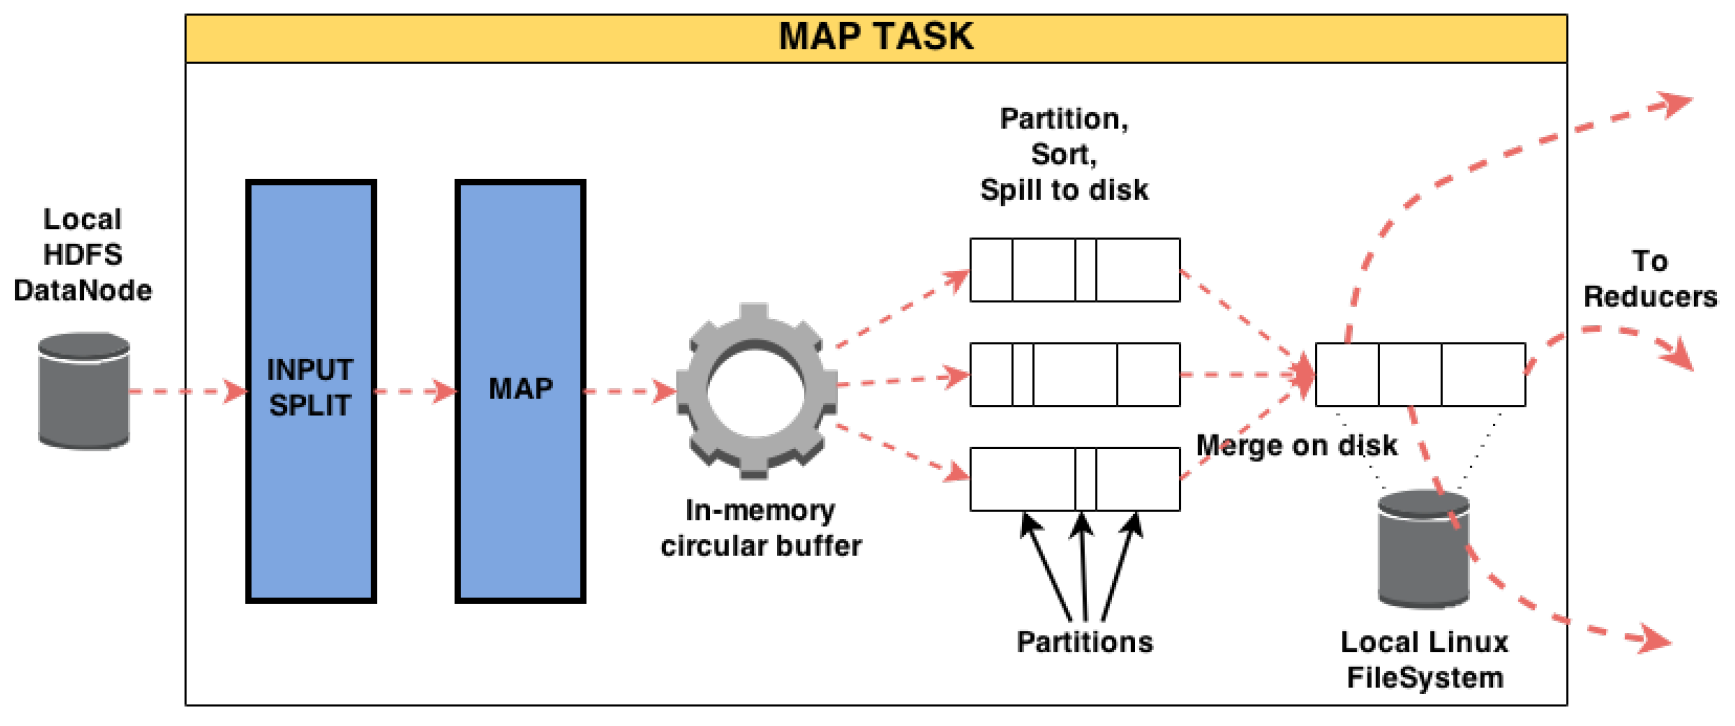
\includegraphics[width=\linewidth]{images/sasmapside.png}
				\caption{\textit{Shuffle and sort: the Map side.}}
			\end{figure}
			\par
			The output of a map task is not simply written to disk, it passes from a circular memory buffer. The buffer has a threshold based mechanism to \textbf{spill} buffer content to disk. The map output is written to the buffer while spilling on disk, if the buffer fills up while spilling the map task is blocked.
			\newline
			The disk spills are written in round-robin to a local directory. The output data are partitioned corresponding to the reducers they will be sent to, within ieach partition, data is \textbf{sorted in memory}.
			\newline
			Optionally, if there is a combiner, it is executed just after the sort phase.
			\newline
			Once the map task finishes there are many spills, such spills are merged into a single, partitioned, and sorted out file.
		\subsection{Shuffle and sort: Reduce side}
			\par
			The map output file is located on the local disk of a TaskTracker. Another TaskTracker (in charge of a reduce task) requires input from many other TaskTracker (that finished their map tasks).
			\newline
			When a map task finishes, it notifies the parent TaskTracker. The parent TaskTracker notifies (heartbeat) the JobTracker. A thread in the reducer polls periodically the JobTracker. TaskTrackers do not delete local map output as soon as a reduce task has fetched them (reliability).
			\begin{figure}[h!]
				\centering
				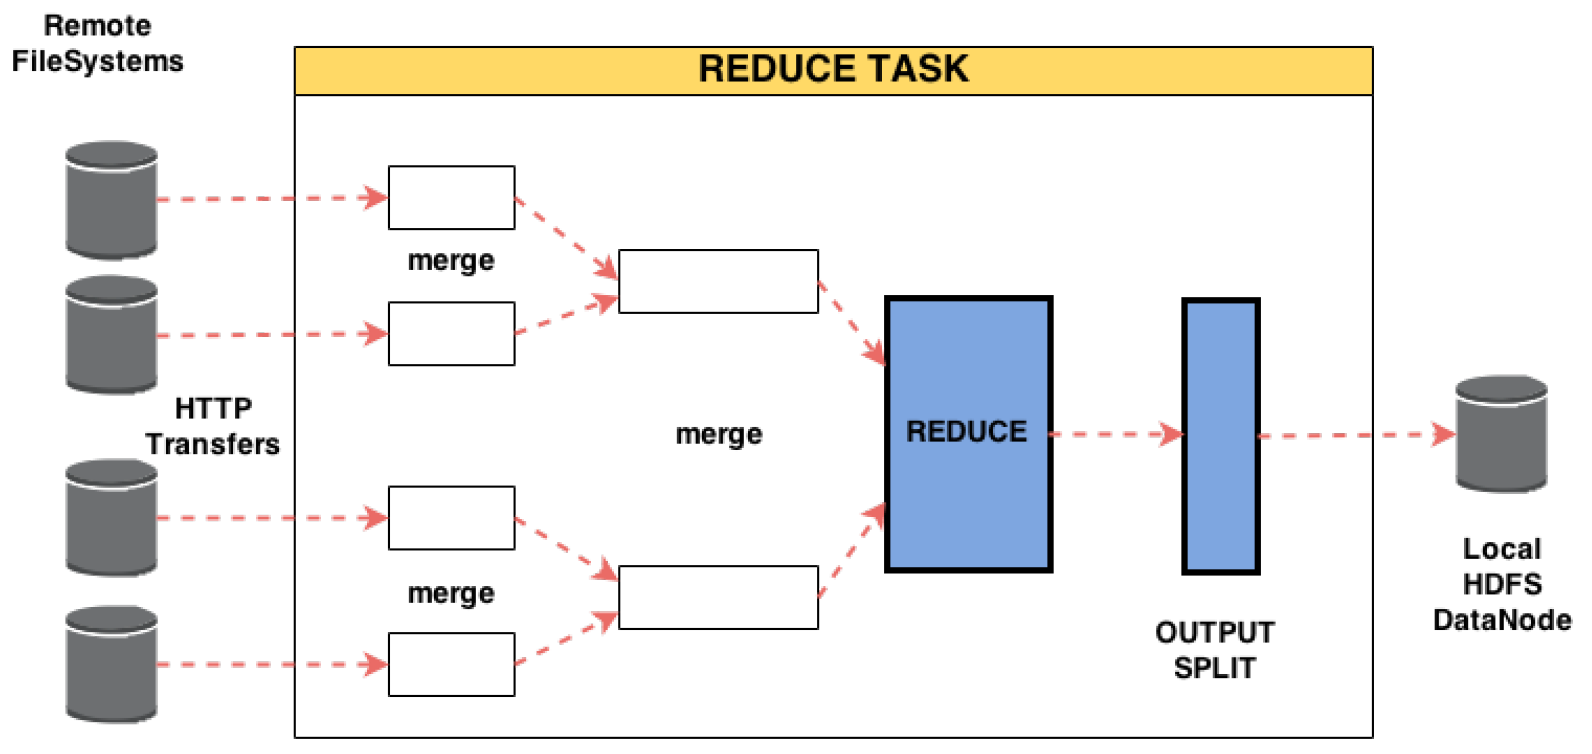
\includegraphics[width=\linewidth]{images/sasreduceside.png}
				\caption{\textit{Shuffle and sort: the Reduce side.}}
			\end{figure}
			\par
			There is a small number of copy threads that can fetch map outputs in parallel. The map output is copied to the TaskTracker running the reducer \textbf{in memory} (if they fit, otherwise they are copied on disk).
			\newline
			A background thread merges all partial inputs into larger, \textbf{sorted} files.